\StartOf{Lecture 14}

\Today{Probability of Error (1) QAM / PSK  examples, (2) FSK, (3) Differential PSK}


\subsection{QAM/PSK Probability of Error Examples}
\Example{Probability of Error in $M$-PSK}

Find the probability of error in $M$-ary PSK using the nearest neighbor approximation.  Is this the same as the union bound?

\vspace{0.1in}
\Solution{
Here the distance between two neighboring symbols can be calculated by seeing the origin and the two symbol points as forming an isosceles triangle with top angle $2\pi/M$, and equal sides having length $A$.  Thus the length of the base is $d_{min} = 2A\sin \frac{2\pi}{2M}$.  The squared distance is
\[
d_{min}^2 = 4A^2 \sin^2 (\pi/M)
\]

The average energy per symbol is simply $A^2$ because all of the symbol points are $A$ from the origin.  Thus the average energy per bit is $\En_b = A^2 / \log_2 M$.  Thus $A^2 = \En_b \log_2 M$.  So:
\[
d_{min}^2 = 4\En_b (\log_2 M ) \sin^2 (\pi/M)
\]

Using the expression for the nearest neighbor approximation:
\begin{eqnarray} \label{E:MPSK_Perror_approx}
  \PR{\mbox{symbol error}} &\approx & \frac{N_{min}}{M}  \Q{\sqrt{\frac{d^2_{min}}{2N_0}}} \nnn
  &\approx& \frac{2M}{M} \Q{\sqrt{4 (\log_2 M)\sin^2 ( \pi/M ) \frac{\En_b }{2N_0}}} \nnn
    &\approx& 2 \Q{\sqrt{2 (\log_2 M)\sin^2 ( \pi/M ) \frac{\En_b }{N_0}}} \nn
\end{eqnarray}

This is the same as the union bound because each symbol only has two neighbors (symbols that contribute to the decision boundary). 
}

The Rice book, Section 6.2, page 319-321, derives an approximate formula for the probability of error in $M$-PSK for $M>4$.  (Recall QPSK has an exact solution.)  For $M>4$, the book shows how to use a polar transformation and approximate the probability of error integral.  The solution is exactly the same, in the end, as the nearest neighbor approximation / union bound expression in (\ref{E:MPSK_Perror_approx}).  




\Example{Additional QAM / PSK Constellations}

Solve for the probability of symbol error in the completely made up signal space diagrams in
Figure \ref{F:exampleQAM-PSK-diagrams}.  You should calculate:
\begin{itemize}
  \item An exact expression if one should happen to be available,
  \item The union bound,
  \item The nearest-neighbor approximation.
\end{itemize}
Solve for the probability of symbol error first, and next the probability of
bit error.  Figure \ref{F:exampleQAM-PSK-diagrams} is in terms of amplitude $A$, but all
probability of error expressions should be written in terms of
$\En_b/N_0$.

\begin{figure}[htbp]
  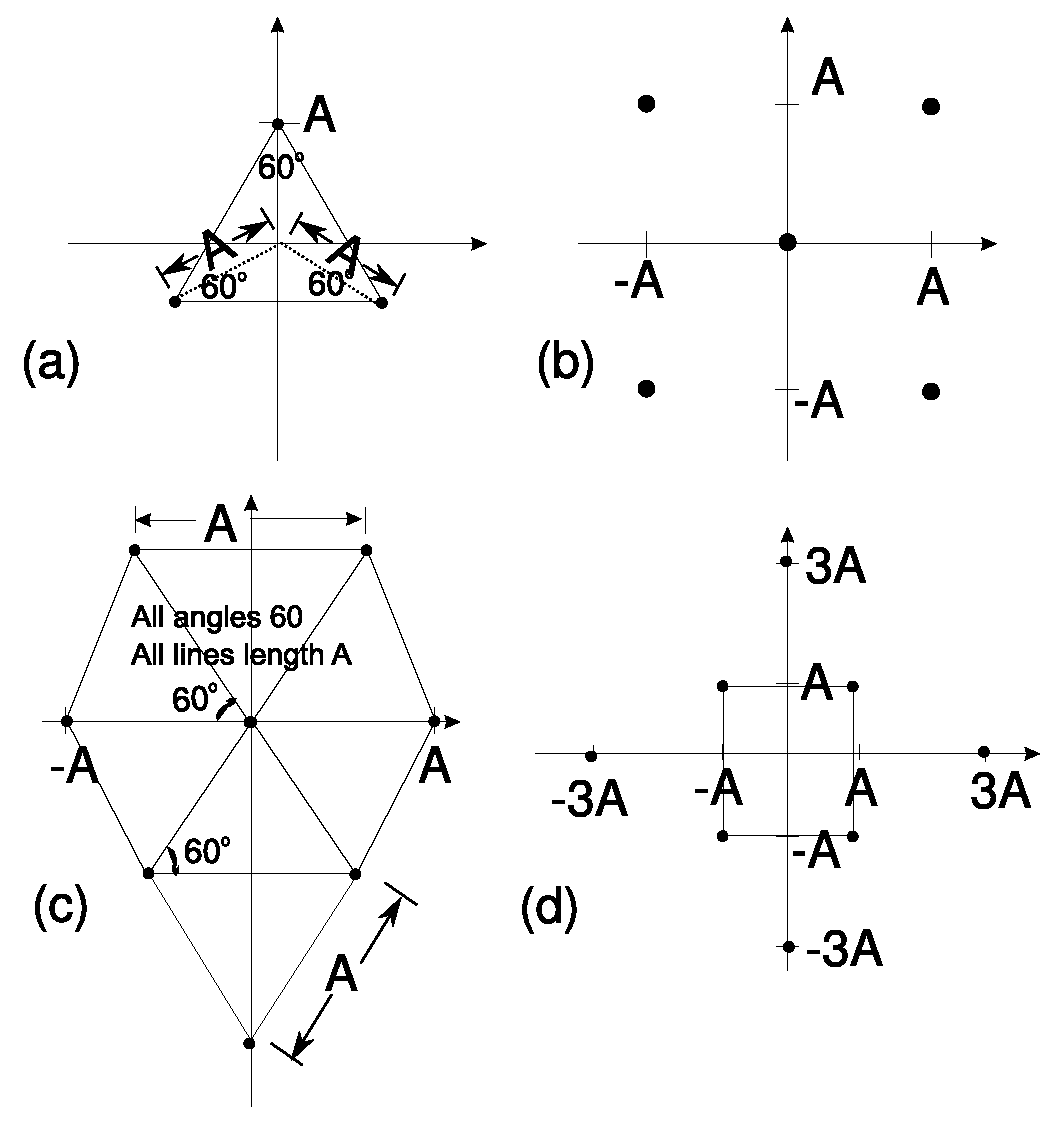
\includegraphics[width=0.9\textwidth]{../images/EgQAM_v2.eps}
  \caption{Constellation diagram for some example (made up) modulations.
  \label{F:exampleQAM-PSK-diagrams}}
\end{figure}
\begin{figure}[htbp]
  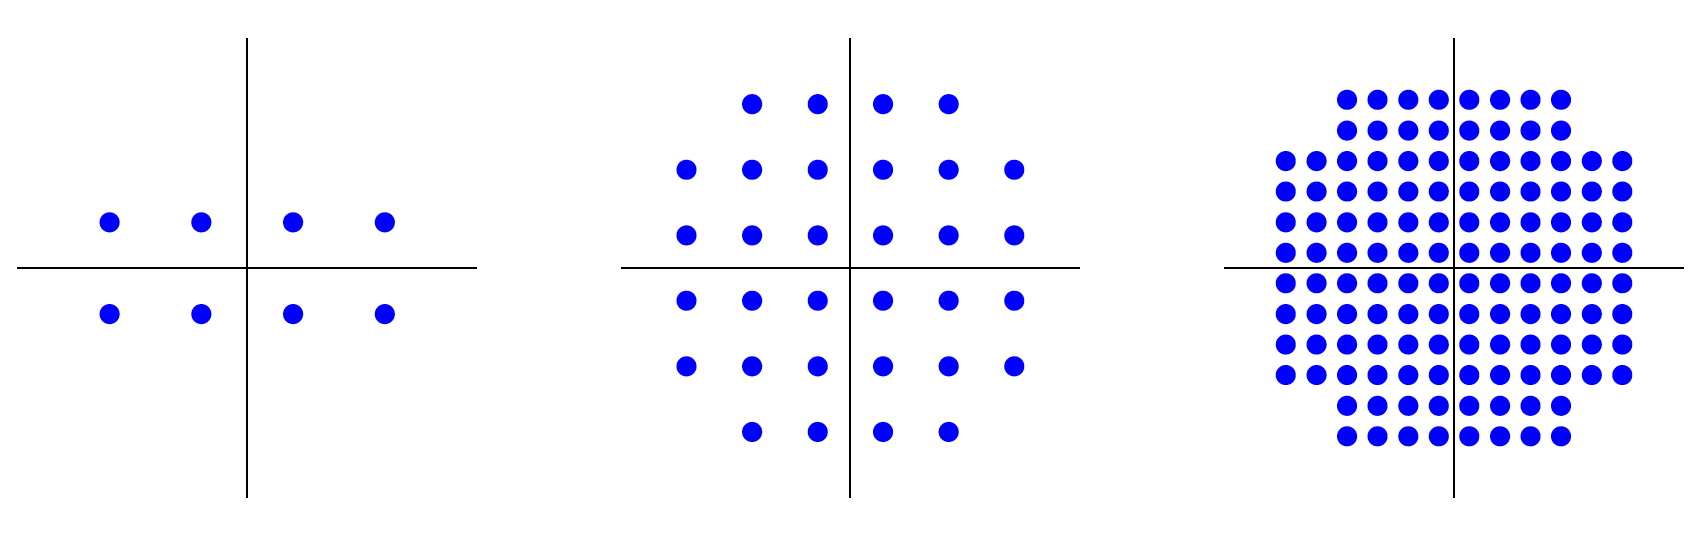
\includegraphics[width=1.0\textwidth]{../images/cross_mqam_8_32_64.png}
  \caption{Constellation diagrams for Cross M-QAM for (left) $M=8$, (center) $M=32$, and (right) $M=64$, from Rice Figure 5.3.4.
  \label{F:exampleCrossQAM}}
\end{figure}

\Example{2 by 4 grid QAM}
Solve for the probability of symbol error in the signal space diagrams in
Rice Figure 5.3.4 (a), copied in these notes as Figure \ref{F:exampleCrossQAM} (left).  You should calculate:
\begin{itemize}
  \item An exact expression,
  \item The union bound,
  \item The nearest-neighbor approximation.
\end{itemize}

\Solution{(a) An exact expression is possible because the decision is separable.  That is, the $x_0$ will decide two of the three bits, while $x_1$ will decide the third bit.  Assume that nearest neighbors are separated by 2A.  For the third bit, the probability of error is that of bipolar PAM, that is, $\Q{\sqrt{\frac{2 A^2}{N_0}}}$.  For the first two bits, the probability of bit error is approximately (assuming Gray coding),
\[
\frac{1}{\log_2 M} \frac{2(M-1)}{M} \Q{\sqrt{\frac{2 A^2}{N_0}}} =  \frac{3}{4} \Q{\sqrt{\frac{2 A^2}{N_0}}}  
\]
The overall average probability of error will be a weighted average of these two -- 2/3 times the probability of bit error in the first two bits and 1/3 times the probability of bit error in the third bit,
\[
 \PR{\mbox{bit error}} \approx \left[ \frac{2}{3}\frac{3}{4}+ \frac{1}{3}\right] \Q{\sqrt{\frac{2 A^2}{N_0}}} = \frac{5}{6}\Q{\sqrt{\frac{2 A^2}{N_0}}}
\]
The average bit energy is 
\begin{eqnarray}
 \En_b &=& \frac{1}{\log_2 8} \En_s\\
 &=& \frac{1}{\log_2 8} \frac{1}{8}\left[ 4(2A^2) + 4*(A^2 + 9A^2)\right] = 2A^2
\end{eqnarray}
Thus 
\[
 \PR{\mbox{bit error}} = \frac{5}{6}\Q{\sqrt{\frac{\En_b}{ N_0}}}
\]

The union bound for (a) and the nearest neighbor approximation are the same.  All nearest neighbors are separated by distance 2A.  Four nodes have two neighbors, and four nodes have three neighbors.  So $N_{min} = 20$, and $d_{min}=2A$. 
So,
\begin{eqnarray} 
  \PR{\mbox{symbol error}}  &\le & \frac{20}{8} \Q{\sqrt{\frac{4A^2}{2N_0}}} = 2.5 \Q{\sqrt{\frac{\En_b}{N_0}}} \nonumber
\end{eqnarray}
Note that this results in an approximate bit error rate of $\frac{5}{6} \Q{\sqrt{\frac{\En_b}{N_0}}}$, the same expression as above.}

\Example{Cross $M=32$ QAM}
Solve for the probability of symbol error in the signal space diagrams in
Rice Figure 5.3.4 (b), copied to these notes as Figure \ref{F:exampleCrossQAM} (center).  You should calculate:
\begin{itemize}
  \item The union bound, and
  \item The nearest-neighbor approximation.
\end{itemize}

\Solution{
The union bound requires us to count neighbors. Assume all nearest neighbors are separated by distance 2A.  
\begin{enumerate}
 \item Sixteen nodes (the center 4x4 grid) have four neighbors at distance $2A$,
 \item Eight nodes have three neighbors at distance $2A$,
 \item Eight nodes have two neighbors at distance $2A$ and one neighbor at distance $2\sqrt{2}A$.  
\end{enumerate}
Also, the average symbol energy is $\frac{1}{32}$ times twice the sum of the squared x-coordinates because of the symmetry of the constellation.
\[
 \En_s = \frac{2(12A^2 + 12(9A^2) + 8(25A^2))}{32} = 20A^2
\]
Since $\log_2 M = 5$, we have $\En_b = \frac{\En_s}{5}  =  4A^2$.
\begin{eqnarray} 
  \PR{\mbox{symbol error}}  &\le & \frac{1}{32} \left\{ (16(4)+8(3)+8(2)) \Q{\sqrt{\frac{4A^2}{2N_0}}} + 8\Q{\sqrt{\frac{8A^2}{2N_0}}} \right\} \nnn
  &\le& \frac{13}{4}\Q{\sqrt{\frac{\En_b}{2 N_0}}} + \frac{1}{4}\Q{\sqrt{\frac{\En_b}{N_0}}}
\end{eqnarray}
The nearest neighbor approximation would simply remove the second term and replace the $\le$ with an $\approx$.
}





\section{FSK Probability of Error}

\subsection{Probability of Error for Coherent Binary FSK}

First, let's look at coherent detection of binary FSK.
\begin{enumerate}
 \item What is the detection threshold line separating the two decision
regions?
 \item What is the distance between points in the Binary FSK signal space?
\end{enumerate}
What is the probability of error for coherent binary FSK?  It
is the same as bipolar PAM, but the symbols are spaced differently (more closely) as a function of $\En_b$.  We had that
\[
\PR{\mbox{error}}_{2-ary} = \Q{\sqrt{\frac{d_{0,1}^2}{2N_0}}}
\]
Now, the spacing between symbols has reduced by a factor of $\sqrt{2}/2$ compared to bipolar PAM, to $d_{0,1} = \sqrt{2\En_b}$.  So
\[
\PR{\mbox{error}}_{2-Co-FSK} = \Q{\sqrt{\frac{\En_b}{N_0}}}
\]
For the same probability of bit error, binary FSK is about 1.5 dB better than OOK (requires 1.5 dB less energy per bit), but 1.5 dB worse than bipolar PAM (requires 1.5 dB more energy per bit).


\begin{figure}[htbp]
  (a) 


\tikzset{every picture/.style={line width=0.75pt}} %set default line width to 0.75pt        

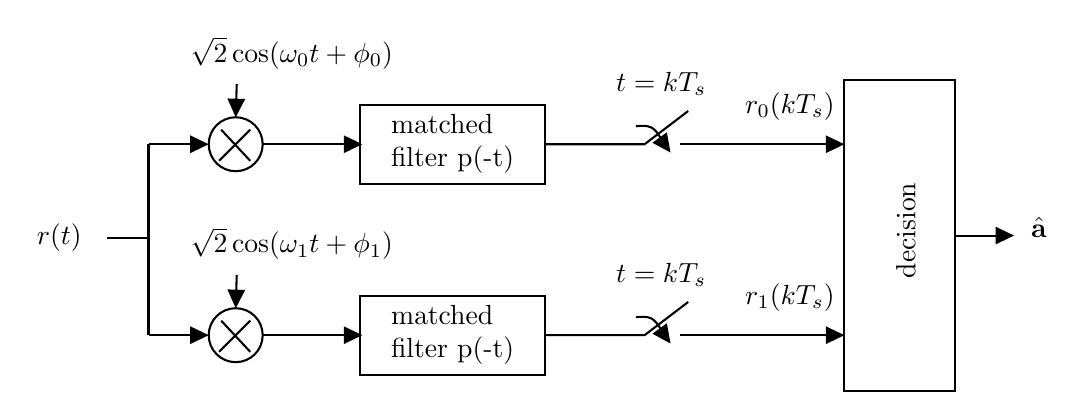
\begin{tikzpicture}[x=0.75pt,y=0.75pt,yscale=-1,xscale=1]
%uncomment if require: \path (0,378); %set diagram left start at 0, and has height of 378

%Straight Lines [id:da015204313020472648] 
\draw    (100,127) -- (120,127) ;
%Straight Lines [id:da3807433535655065] 
\draw    (120,174) -- (120,82) ;
%Straight Lines [id:da13452699900895748] 
\draw    (120,82) -- (146,82) ;
\draw [shift={(149,82)}, rotate = 180] [fill={rgb, 255:red, 0; green, 0; blue, 0 }  ][line width=0.08]  [draw opacity=0] (8.93,-4.29) -- (0,0) -- (8.93,4.29) -- cycle    ;
%Shape: Rectangle [id:dp6831503614766208] 
\draw   (222,63) -- (311,63) -- (311,101) -- (222,101) -- cycle ;
%Shape: Circle [id:dp5132093237924611] 
\draw   (149,82) .. controls (149,74.82) and (154.82,69) .. (162,69) .. controls (169.18,69) and (175,74.82) .. (175,82) .. controls (175,89.18) and (169.18,95) .. (162,95) .. controls (154.82,95) and (149,89.18) .. (149,82) -- cycle ;
%Straight Lines [id:da25287195023205933] 
\draw    (155,75) -- (169,90) ;
%Straight Lines [id:da5242592168562576] 
\draw    (169,75) -- (154,90) ;
%Straight Lines [id:da23051729614765581] 
\draw    (162.09,66) -- (162.5,53) ;
\draw [shift={(162,69)}, rotate = 271.79] [fill={rgb, 255:red, 0; green, 0; blue, 0 }  ][line width=0.08]  [draw opacity=0] (8.93,-4.29) -- (0,0) -- (8.93,4.29) -- cycle    ;
%Straight Lines [id:da2971482914437682] 
\draw    (175,82) -- (220,82) ;
\draw [shift={(223,82)}, rotate = 180] [fill={rgb, 255:red, 0; green, 0; blue, 0 }  ][line width=0.08]  [draw opacity=0] (8.93,-4.29) -- (0,0) -- (8.93,4.29) -- cycle    ;
%Straight Lines [id:da24289517343868772] 
\draw    (311,82) -- (359,82) -- (380,66) ;
%Straight Lines [id:da03913348203652922] 
\draw    (376,82) -- (452.24,82) ;
\draw [shift={(455.24,82)}, rotate = 180] [fill={rgb, 255:red, 0; green, 0; blue, 0 }  ][line width=0.08]  [draw opacity=0] (8.93,-4.29) -- (0,0) -- (8.93,4.29) -- cycle    ;
%Curve Lines [id:da6656366911860763] 
\draw    (354.83,73.33) .. controls (364.08,72.41) and (363.64,74.62) .. (369.85,83.66) ;
\draw [shift={(371.5,86)}, rotate = 233.97] [fill={rgb, 255:red, 0; green, 0; blue, 0 }  ][line width=0.08]  [draw opacity=0] (8.93,-4.29) -- (0,0) -- (8.93,4.29) -- cycle    ;
%Shape: Rectangle [id:dp38931328167896195] 
\draw   (455.24,51) -- (508.5,51) -- (508.5,201) -- (455.24,201) -- cycle ;
%Straight Lines [id:da5073149386864682] 
\draw    (508,126) -- (534,126) ;
\draw [shift={(537,126)}, rotate = 180] [fill={rgb, 255:red, 0; green, 0; blue, 0 }  ][line width=0.08]  [draw opacity=0] (8.93,-4.29) -- (0,0) -- (8.93,4.29) -- cycle    ;
%Straight Lines [id:da0935600260327849] 
\draw    (120,174) -- (146,174) ;
\draw [shift={(149,174)}, rotate = 180] [fill={rgb, 255:red, 0; green, 0; blue, 0 }  ][line width=0.08]  [draw opacity=0] (8.93,-4.29) -- (0,0) -- (8.93,4.29) -- cycle    ;
%Shape: Rectangle [id:dp5397600807528802] 
\draw   (222,155) -- (311,155) -- (311,193) -- (222,193) -- cycle ;
%Shape: Circle [id:dp6340079603545306] 
\draw   (149,174) .. controls (149,166.82) and (154.82,161) .. (162,161) .. controls (169.18,161) and (175,166.82) .. (175,174) .. controls (175,181.18) and (169.18,187) .. (162,187) .. controls (154.82,187) and (149,181.18) .. (149,174) -- cycle ;
%Straight Lines [id:da054936665320719724] 
\draw    (155,167) -- (169,182) ;
%Straight Lines [id:da14446384117365363] 
\draw    (169,167) -- (154,182) ;
%Straight Lines [id:da06806069680494597] 
\draw    (162.09,158) -- (162.5,145) ;
\draw [shift={(162,161)}, rotate = 271.79] [fill={rgb, 255:red, 0; green, 0; blue, 0 }  ][line width=0.08]  [draw opacity=0] (8.93,-4.29) -- (0,0) -- (8.93,4.29) -- cycle    ;
%Straight Lines [id:da13918324188613052] 
\draw    (175,174) -- (220,174) ;
\draw [shift={(223,174)}, rotate = 180] [fill={rgb, 255:red, 0; green, 0; blue, 0 }  ][line width=0.08]  [draw opacity=0] (8.93,-4.29) -- (0,0) -- (8.93,4.29) -- cycle    ;
%Straight Lines [id:da7726545291977289] 
\draw    (311,174) -- (359,174) -- (380,158) ;
%Straight Lines [id:da5999576449313313] 
\draw    (376,174) -- (452.24,174) ;
\draw [shift={(455.24,174)}, rotate = 180] [fill={rgb, 255:red, 0; green, 0; blue, 0 }  ][line width=0.08]  [draw opacity=0] (8.93,-4.29) -- (0,0) -- (8.93,4.29) -- cycle    ;
%Curve Lines [id:da38919606803399187] 
\draw    (354.83,165.33) .. controls (364.08,164.41) and (363.64,166.62) .. (369.85,175.66) ;
\draw [shift={(371.5,178)}, rotate = 233.97] [fill={rgb, 255:red, 0; green, 0; blue, 0 }  ][line width=0.08]  [draw opacity=0] (8.93,-4.29) -- (0,0) -- (8.93,4.29) -- cycle    ;

% Text Node
\draw (189,38) node    {$\sqrt{2}\cos( \omega _{0} t+\phi _{0})$};
% Text Node
\draw (266.5,82) node   [align=left] {matched\\filter p(-t)};
% Text Node
\draw (367,53) node    {$t=kT_{s}$};
% Text Node
\draw (429,64) node    {$r_{0}( kT_{s})$};
% Text Node
\draw (484.87,123.5) node  [rotate=-269.97] [align=left] {decision};
% Text Node
\draw (549,122) node    {$\hat{\mathbf{a}}$};
% Text Node
\draw (77,127) node    {$r( t)$};
% Text Node
\draw (189,130) node    {$\sqrt{2}\cos( \omega _{1} t+\phi _{1})$};
% Text Node
\draw (266.5,174) node   [align=left] {matched\\filter p(-t)};
% Text Node
\draw (367,145) node    {$t=kT_{s}$};
% Text Node
\draw (429,156) node    {$r_{1}( kT_{s})$};


\end{tikzpicture}
  
  (b) 


\tikzset{every picture/.style={line width=0.75pt}} %set default line width to 0.75pt        

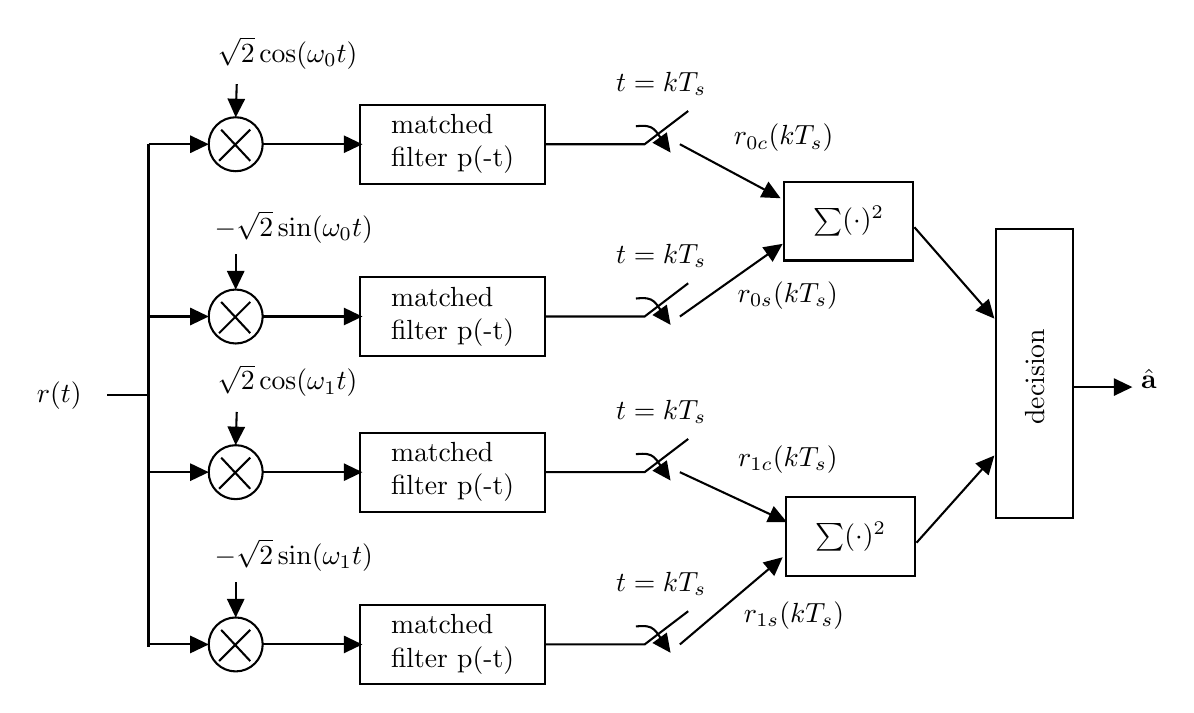
\begin{tikzpicture}[x=0.75pt,y=0.75pt,yscale=-1,xscale=1]
%uncomment if require: \path (0,378); %set diagram left start at 0, and has height of 378

%Straight Lines [id:da015204313020472648] 
\draw    (100,203) -- (120,203) ;
%Straight Lines [id:da3807433535655065] 
\draw    (120,148) -- (120,82) ;
%Straight Lines [id:da13452699900895748] 
\draw    (120,82) -- (146,82) ;
\draw [shift={(149,82)}, rotate = 180] [fill={rgb, 255:red, 0; green, 0; blue, 0 }  ][line width=0.08]  [draw opacity=0] (8.93,-4.29) -- (0,0) -- (8.93,4.29) -- cycle    ;
%Shape: Rectangle [id:dp6831503614766208] 
\draw   (222,63) -- (311,63) -- (311,101) -- (222,101) -- cycle ;
%Shape: Circle [id:dp5132093237924611] 
\draw   (149,82) .. controls (149,74.82) and (154.82,69) .. (162,69) .. controls (169.18,69) and (175,74.82) .. (175,82) .. controls (175,89.18) and (169.18,95) .. (162,95) .. controls (154.82,95) and (149,89.18) .. (149,82) -- cycle ;
%Straight Lines [id:da25287195023205933] 
\draw    (155,75) -- (169,90) ;
%Straight Lines [id:da5242592168562576] 
\draw    (169,75) -- (154,90) ;
%Straight Lines [id:da23051729614765581] 
\draw    (162.09,66) -- (162.5,53) ;
\draw [shift={(162,69)}, rotate = 271.79] [fill={rgb, 255:red, 0; green, 0; blue, 0 }  ][line width=0.08]  [draw opacity=0] (8.93,-4.29) -- (0,0) -- (8.93,4.29) -- cycle    ;
%Straight Lines [id:da2971482914437682] 
\draw    (175,82) -- (220,82) ;
\draw [shift={(223,82)}, rotate = 180] [fill={rgb, 255:red, 0; green, 0; blue, 0 }  ][line width=0.08]  [draw opacity=0] (8.93,-4.29) -- (0,0) -- (8.93,4.29) -- cycle    ;
%Straight Lines [id:da24289517343868772] 
\draw    (311,82) -- (359,82) -- (380,66) ;
%Straight Lines [id:da03913348203652922] 
\draw    (376,82) -- (421.86,106.58) ;
\draw [shift={(424.5,108)}, rotate = 208.19] [fill={rgb, 255:red, 0; green, 0; blue, 0 }  ][line width=0.08]  [draw opacity=0] (8.93,-4.29) -- (0,0) -- (8.93,4.29) -- cycle    ;
%Curve Lines [id:da6656366911860763] 
\draw    (354.83,73.33) .. controls (364.08,72.41) and (363.64,74.62) .. (369.85,83.66) ;
\draw [shift={(371.5,86)}, rotate = 233.97] [fill={rgb, 255:red, 0; green, 0; blue, 0 }  ][line width=0.08]  [draw opacity=0] (8.93,-4.29) -- (0,0) -- (8.93,4.29) -- cycle    ;
%Straight Lines [id:da8443900724542854] 
\draw    (120,166) -- (120,100) ;
%Straight Lines [id:da5599679464635203] 
\draw    (120,165) -- (146,165) ;
\draw [shift={(149,165)}, rotate = 180] [fill={rgb, 255:red, 0; green, 0; blue, 0 }  ][line width=0.08]  [draw opacity=0] (8.93,-4.29) -- (0,0) -- (8.93,4.29) -- cycle    ;
%Shape: Rectangle [id:dp4728769628725722] 
\draw   (222,146) -- (311,146) -- (311,184) -- (222,184) -- cycle ;
%Shape: Circle [id:dp6949030494745931] 
\draw   (149,165) .. controls (149,157.82) and (154.82,152) .. (162,152) .. controls (169.18,152) and (175,157.82) .. (175,165) .. controls (175,172.18) and (169.18,178) .. (162,178) .. controls (154.82,178) and (149,172.18) .. (149,165) -- cycle ;
%Straight Lines [id:da04939422211851974] 
\draw    (155,158) -- (169,173) ;
%Straight Lines [id:da5057896656126377] 
\draw    (169,158) -- (154,173) ;
%Straight Lines [id:da2187796485955027] 
\draw    (162,149) -- (162,135.01) ;
\draw [shift={(162,152)}, rotate = 270] [fill={rgb, 255:red, 0; green, 0; blue, 0 }  ][line width=0.08]  [draw opacity=0] (8.93,-4.29) -- (0,0) -- (8.93,4.29) -- cycle    ;
%Straight Lines [id:da682896982719438] 
\draw    (175,165) -- (220,165) ;
\draw [shift={(223,165)}, rotate = 180] [fill={rgb, 255:red, 0; green, 0; blue, 0 }  ][line width=0.08]  [draw opacity=0] (8.93,-4.29) -- (0,0) -- (8.93,4.29) -- cycle    ;
%Straight Lines [id:da5718199074050085] 
\draw    (311,165) -- (359,165) -- (380,149) ;
%Straight Lines [id:da5343223302986524] 
\draw    (376,165) -- (423.05,131.73) ;
\draw [shift={(425.5,130)}, rotate = 504.74] [fill={rgb, 255:red, 0; green, 0; blue, 0 }  ][line width=0.08]  [draw opacity=0] (8.93,-4.29) -- (0,0) -- (8.93,4.29) -- cycle    ;
%Curve Lines [id:da12127995754356569] 
\draw    (354.83,156.33) .. controls (364.08,155.41) and (363.64,157.62) .. (369.85,166.66) ;
\draw [shift={(371.5,169)}, rotate = 233.97] [fill={rgb, 255:red, 0; green, 0; blue, 0 }  ][line width=0.08]  [draw opacity=0] (8.93,-4.29) -- (0,0) -- (8.93,4.29) -- cycle    ;
%Shape: Rectangle [id:dp38931328167896195] 
\draw   (528.24,123) -- (565.5,123) -- (565.5,262) -- (528.24,262) -- cycle ;
%Straight Lines [id:da5073149386864682] 
\draw    (565,199) -- (591,199) ;
\draw [shift={(594,199)}, rotate = 180] [fill={rgb, 255:red, 0; green, 0; blue, 0 }  ][line width=0.08]  [draw opacity=0] (8.93,-4.29) -- (0,0) -- (8.93,4.29) -- cycle    ;
%Straight Lines [id:da15082826510468084] 
\draw    (120,306) -- (120,240) ;
%Straight Lines [id:da0935600260327849] 
\draw    (120,240) -- (146,240) ;
\draw [shift={(149,240)}, rotate = 180] [fill={rgb, 255:red, 0; green, 0; blue, 0 }  ][line width=0.08]  [draw opacity=0] (8.93,-4.29) -- (0,0) -- (8.93,4.29) -- cycle    ;
%Shape: Rectangle [id:dp5397600807528802] 
\draw   (222,221) -- (311,221) -- (311,259) -- (222,259) -- cycle ;
%Shape: Circle [id:dp6340079603545306] 
\draw   (149,240) .. controls (149,232.82) and (154.82,227) .. (162,227) .. controls (169.18,227) and (175,232.82) .. (175,240) .. controls (175,247.18) and (169.18,253) .. (162,253) .. controls (154.82,253) and (149,247.18) .. (149,240) -- cycle ;
%Straight Lines [id:da054936665320719724] 
\draw    (155,233) -- (169,248) ;
%Straight Lines [id:da14446384117365363] 
\draw    (169,233) -- (154,248) ;
%Straight Lines [id:da06806069680494597] 
\draw    (162.09,224) -- (162.5,211) ;
\draw [shift={(162,227)}, rotate = 271.79] [fill={rgb, 255:red, 0; green, 0; blue, 0 }  ][line width=0.08]  [draw opacity=0] (8.93,-4.29) -- (0,0) -- (8.93,4.29) -- cycle    ;
%Straight Lines [id:da13918324188613052] 
\draw    (175,240) -- (220,240) ;
\draw [shift={(223,240)}, rotate = 180] [fill={rgb, 255:red, 0; green, 0; blue, 0 }  ][line width=0.08]  [draw opacity=0] (8.93,-4.29) -- (0,0) -- (8.93,4.29) -- cycle    ;
%Straight Lines [id:da7726545291977289] 
\draw    (311,240) -- (359,240) -- (380,224) ;
%Straight Lines [id:da5999576449313313] 
\draw    (376,240) -- (424.78,262.73) ;
\draw [shift={(427.5,264)}, rotate = 204.99] [fill={rgb, 255:red, 0; green, 0; blue, 0 }  ][line width=0.08]  [draw opacity=0] (8.93,-4.29) -- (0,0) -- (8.93,4.29) -- cycle    ;
%Curve Lines [id:da38919606803399187] 
\draw    (354.83,231.33) .. controls (364.08,230.41) and (363.64,232.62) .. (369.85,241.66) ;
\draw [shift={(371.5,244)}, rotate = 233.97] [fill={rgb, 255:red, 0; green, 0; blue, 0 }  ][line width=0.08]  [draw opacity=0] (8.93,-4.29) -- (0,0) -- (8.93,4.29) -- cycle    ;
%Straight Lines [id:da8734795030480866] 
\draw    (120,324) -- (120,258) ;
%Straight Lines [id:da8040116363807426] 
\draw    (120,323) -- (146,323) ;
\draw [shift={(149,323)}, rotate = 180] [fill={rgb, 255:red, 0; green, 0; blue, 0 }  ][line width=0.08]  [draw opacity=0] (8.93,-4.29) -- (0,0) -- (8.93,4.29) -- cycle    ;
%Shape: Rectangle [id:dp5975491454430302] 
\draw   (222,304) -- (311,304) -- (311,342) -- (222,342) -- cycle ;
%Shape: Circle [id:dp7916200903945911] 
\draw   (149,323) .. controls (149,315.82) and (154.82,310) .. (162,310) .. controls (169.18,310) and (175,315.82) .. (175,323) .. controls (175,330.18) and (169.18,336) .. (162,336) .. controls (154.82,336) and (149,330.18) .. (149,323) -- cycle ;
%Straight Lines [id:da611405707361617] 
\draw    (155,316) -- (169,331) ;
%Straight Lines [id:da2122883053855653] 
\draw    (169,316) -- (154,331) ;
%Straight Lines [id:da8750328174207926] 
\draw    (162,307) -- (162,293.01) ;
\draw [shift={(162,310)}, rotate = 270] [fill={rgb, 255:red, 0; green, 0; blue, 0 }  ][line width=0.08]  [draw opacity=0] (8.93,-4.29) -- (0,0) -- (8.93,4.29) -- cycle    ;
%Straight Lines [id:da8948341846863821] 
\draw    (175,323) -- (220,323) ;
\draw [shift={(223,323)}, rotate = 180] [fill={rgb, 255:red, 0; green, 0; blue, 0 }  ][line width=0.08]  [draw opacity=0] (8.93,-4.29) -- (0,0) -- (8.93,4.29) -- cycle    ;
%Straight Lines [id:da08761812164421467] 
\draw    (311,323) -- (359,323) -- (380,307) ;
%Straight Lines [id:da5444101654646902] 
\draw    (376,323) -- (423.21,282.94) ;
\draw [shift={(425.5,281)}, rotate = 499.69] [fill={rgb, 255:red, 0; green, 0; blue, 0 }  ][line width=0.08]  [draw opacity=0] (8.93,-4.29) -- (0,0) -- (8.93,4.29) -- cycle    ;
%Curve Lines [id:da9988843661394544] 
\draw    (354.83,314.33) .. controls (364.08,313.41) and (363.64,315.62) .. (369.85,324.66) ;
\draw [shift={(371.5,327)}, rotate = 233.97] [fill={rgb, 255:red, 0; green, 0; blue, 0 }  ][line width=0.08]  [draw opacity=0] (8.93,-4.29) -- (0,0) -- (8.93,4.29) -- cycle    ;
%Straight Lines [id:da18833199394628286] 
\draw    (120,166) -- (120,240) ;
%Shape: Rectangle [id:dp5041141748535656] 
\draw   (426,100) -- (488.5,100) -- (488.5,138) -- (426,138) -- cycle ;
%Straight Lines [id:da5457056539898697] 
\draw    (489,122) -- (525.52,163.74) ;
\draw [shift={(527.5,166)}, rotate = 228.81] [fill={rgb, 255:red, 0; green, 0; blue, 0 }  ][line width=0.08]  [draw opacity=0] (8.93,-4.29) -- (0,0) -- (8.93,4.29) -- cycle    ;
%Shape: Rectangle [id:dp7999711344739604] 
\draw   (427,252) -- (489.5,252) -- (489.5,290) -- (427,290) -- cycle ;
%Straight Lines [id:da15975657015750078] 
\draw    (490,274) -- (525.5,234.24) ;
\draw [shift={(527.5,232)}, rotate = 491.76] [fill={rgb, 255:red, 0; green, 0; blue, 0 }  ][line width=0.08]  [draw opacity=0] (8.93,-4.29) -- (0,0) -- (8.93,4.29) -- cycle    ;

% Text Node
\draw (187,38) node    {$\sqrt{2}\cos( \omega _{0} t)$};
% Text Node
\draw (266.5,82) node   [align=left] {matched\\filter p(-t)};
% Text Node
\draw (367,53) node    {$t=kT_{s}$};
% Text Node
\draw (426,79) node    {$r_{0c}( kT_{s})$};
% Text Node
\draw (190,122) node    {$-\sqrt{2}\sin( \omega _{0} t)$};
% Text Node
\draw (266.5,165) node   [align=left] {matched\\filter p(-t)};
% Text Node
\draw (367,136) node    {$t=kT_{s}$};
% Text Node
\draw (428,155) node    {$r_{0s}( kT_{s})$};
% Text Node
\draw (546.87,194) node  [rotate=-269.97] [align=left] {decision};
% Text Node
\draw (602,195) node    {$\hat{\mathbf{a}}$};
% Text Node
\draw (77,203) node    {$r( t)$};
% Text Node
\draw (187,196) node    {$\sqrt{2}\cos( \omega _{1} t)$};
% Text Node
\draw (266.5,240) node   [align=left] {matched\\filter p(-t)};
% Text Node
\draw (367,211) node    {$t=kT_{s}$};
% Text Node
\draw (428,234) node    {$r_{1c}( kT_{s})$};
% Text Node
\draw (190,280) node    {$-\sqrt{2}\sin( \omega _{1} t)$};
% Text Node
\draw (266.5,323) node   [align=left] {matched\\filter p(-t)};
% Text Node
\draw (367,294) node    {$t=kT_{s}$};
% Text Node
\draw (431,309) node    {$r_{1s}( kT_{s})$};
% Text Node
\draw (457.25,119) node    {$\sum ( \cdot )^{2}$};
% Text Node
\draw (458.25,271) node    {$\sum ( \cdot )^{2}$};


\end{tikzpicture}
  
  \caption{Block diagram of receivers for binary FSK. (a) A coherent RX synchronizes to the phases $\phi_0$, $\phi_1$ of the cosines at each frequency $\omega_0$, $\omega_1$, correlates with the two possible waveforms, and then decides which of the two symbols is closest.  (b) A non-coherent RX does not try to estimate the phases, and instead, correlates with a cosine and a sine at each frequency $\omega_0$ and $\omega_1$, computes the energy in band $m$ as $r_{mc}^2 + r_{ms}^2$, and finds which one has the highest energy.
  \label{F:FSK_block_diagrams}}
\end{figure}

\subsection{Probability of Error for Noncoherent Binary FSK}

The energy detector uses the energy in each frequency and selects the frequency with maximum energy.

This energy is denoted $r_m^2$ for frequency $m\in \{0,1\}$ and is
\[
 r_m^2 = r_{mc}^2 + r_{ms}^2
\]
This energy measure is a statistic which measures how much energy
was in the signal at frequency $f_m$.  The `envelope' is a term used
for the square root of the energy, so $r_m$ is termed the envelope.

Question: What will $r_m^2$ equal when the noise is very small?

As it turns out, given the non-coherent receiver and $r_{mc}$ and
$r_{ms}$, the envelope $r_m$ is an optimum (sufficient) statistic to
use to decide between $s_0 \ldots s_{M-1}$.

What do they do to prove this in Proakis \& Salehi?  They prove it for
\emph{binary} non-coherent FSK.  It takes quite a bit to do
this proof; one needs to have some practice in transformations of random variables.  A sketch:
\begin{enumerate}
 \item Define the received vector $\mbr$ as a $4$ length vector of
   the correlation of $r(t)$ with the sin and cos at each frequency $f_0, f_1$.
 \item They formulate the prior probabilities $f_{\mbr | H_i}(\mbr | H_i)$.  Note that
   this depends on $\theta_m$, which is assumed to be uniform between
   $0$ and $2\pi$, and independent of the noise.
   \begin{eqnarray}
     f_{\mbr | H_i}(\mbr | H_i) &=& \int_0^{2\pi} f_{\mbr,\theta_m | H_i}(\mbr,\phi |
     H_i) d\phi \nonumber \\
         &=& \int_0^{2\pi} f_{\mbr | \theta_m, H_i}(\mbr | \phi, H_i) f_{\theta_m|H_i}(\phi | H_i) d\phi \nonumber \\
   \end{eqnarray}
   Note that $f_{\mbr |  \theta_m, H_0}(\mbr | \phi, H_0)$ is a 2-D Gaussian random vector with i.i.d. components.
 \item They formulate the joint probabilities $f_{\mbr \cap H_0}(\mbr \cap H_0)$
   and $f_{\mbr \cap H_1}(\mbr \cap H_1)$.
 \item Where the joint probability $f_{\mbr \cap H_0}(\mbr \cap H_0)$ is
   greater than $f_{\mbr| H_1}(\mbr | H_1)$, the receiver decides
   $H_0$.  Otherwise, it decides $H_1$.
 \item The decisions in this last step, after manipulation of the
   pdfs, are shown to reduce to this decision (given that $\PR{H_0} =
   \PR{H_1}$):
   \[
     \sqrt{r_{0c}^2 + r_{0s}^2} \decision{H_0}{H_1} \sqrt{r_{1c}^2 + r_{1s}^2}
   \]
\end{enumerate}
The ``envelope detector'' can equally well be called the ``energy
detector'', and it often is.  The full proof of the probability of error is in Proakis \& Salehi, Section 7.6.9, page 430 (which is posted on Canvas).  The expression for probability of error in binary non-coherent FSK is given by,
\begin{equation} \label{E:2-nc-fsk}
 \PR{\mbox{error}}_{2-NC-FSK} = \frac{1}{2} \exp \left[- \frac{\En_b}{2N_0} \right]
\end{equation}
The expressions for probability of error in binary FSK (both coherent and non-coherent) are important, and you should make note of them.  You will use them to be able to design communication systems that use FSK.





















\section{Differential Coding for BPSK}


%The bandpass signal for PSK is,
%\[
%  s(t) = \cos(2\pi f_c t + \angle \mba_k(t)).
%\]
%for $k=0\ldots M-1$.
%
%
\Definition{Coherent Reception}{The reception of a signal when its
carrier phase is explicitly determined and used for demodulation.}

For coherent reception of PSK, will always need some kind of phase
synchronization in BPSK.   Typically, this means transmitting a
training sequence.

For non-coherent reception of PSK, we use differential encoding (at
the transmitter) and decoding (at the receiver).

\subsection{DPSK Transmitter}

Now, consider the bit sequence $\{b_n\}$, where $b_n$ is the $n$th
bit that we want to send.  The sequence $b_n$ is a sequence of 0's
and 1's. How do we decide which phase to send? Prior to this, we've
said, send $\mba_0$ if $b_n=0$, and send $\mba_1$ if $b_n = 1$.

Instead of setting $k$ for $\mba_k$ only as a function of $b_n$, in
differential encoding, we also include $k_{n-1}$.  Now,
\[
 k_n = \twooptions{k_{n-1}}{b_n=0}{1-k_{n-1}}{b_n=1}
\]
Note that $1-k_{n-1}$ is the complement or negation of $k_{n-1}$ --
if $k_{n-1}=1$ then $1-k_{n-1}=0$; if $k_{n-1}=0$ then
$1-k_{n-1}=1$. Basically, for differential BPSK, a switch in the
angle of the signal space vector from $0^o$ to $180^o$ or vice versa
indicates a bit 1; while staying at the same angle indicates a bit
0.

Note that the TX and RX have to agree on the ``zero'' phase.  Typically
$k_{0}=0$.  This becomes an \emph{extra} bit sent with the data bits.

\Example{Differential encoding}

Let $\mbb = [1, 0, 1, 0, 1, 1, 1, 0, 0 ]$.  Assume $b_0=0$.
 What symbols $\mbk = [ k_0, \ldots, k_9]^T$ will be sent?
\Solution{
\[
\mbk = [0, 1, 1, 0, 0,  1, 0, 1, 1, 1]^T
\]
These values of $k_n$ correspond to a symbol stream with phases:
\[
\angle \mba = [0, \pi, \pi, 0, 0,  \pi, 0, \pi, \pi, \pi]^T
\]

}

\subsection{DPSK Receiver}

Now, at the receiver, we
find $b_n$ by comparing the phase of $x_{n}$ to the phase of $x_{n-1}$.  
What our receiver does, is to measure the angle difference is small (close to zero) or large (bigger than $\pi/2$)
\[
   \cos (\angle x_n - \angle x_{n-1})
\]
If this statistic is less than zero, decide $b_n=1$, and if
it is greater than zero, decide $b_n=0$.


\Example{Differential decoding}
\begin{enumerate}
\item Assuming no phase shift in the above encoding example, show that the receiver
will decode the original bitstream with differential decoding.
\Solution{Starting with the 2nd element of $\angle \mba$ above,
\[
\hat{b}_n = [1, 0, 1, 0, 1, 1, 1, 0, 0 ]^T.
\]
}
 \item Now, assume that all bits are shifted $\pi$ radians and we
 receive
\[
\angle \mbx'   = [\pi, 0, 0, \pi, \pi,  0, \pi, 0, 0, 0].
\]
 What will be decoded at the receiver?
\Solution{
\[
\hat{b}_n = [1, 0, 1,   0,    1,   1, 1, 0, 0 ].
\]
}
\end{enumerate}
Rotating \emph{all} symbols by $\pi$ radians does not cause any bit error.

\subsection{Probability of Bit Error for DPSK}

The probability of bit error in DPSK is slightly worse than that for BPSK:

\[
 \PR{\mbox{error}} = \frac{1}{2} \exp\left( -\Ebno \right) 
\]

For a constant probability of error, DPSK requires about 1 dB more $\Ebno$ than BPSK, which has probability of bit error $\Q{\sqrt{\frac{2\En_b}{N_0}}}$.  Both are plotted in Figure \ref{F:bpsk_vs_dpsk}.

\begin{figure}[htbp]
  \centerline{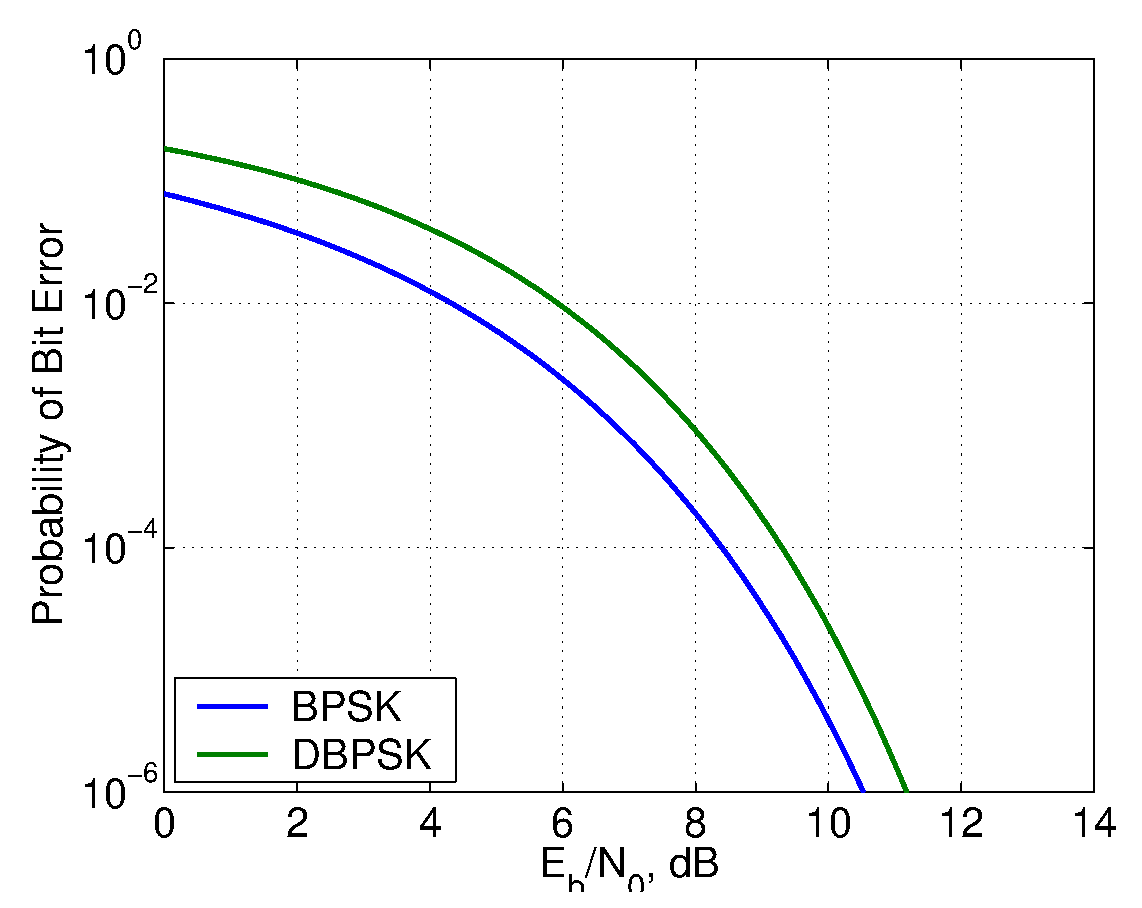
\includegraphics[width=0.65\textwidth]{../images/plotPbiterror_DPSK.eps}}
  \caption{Comparison of probability of bit error for BPSK and Differential BPSK.}
  \label{F:bpsk_vs_dpsk}
\end{figure}

